\documentclass[portrait]{usydposter}
\usepackage{xspace}
\usepackage{graphicx}

\newcommand{\acronym}[1]{\textsc{#1}\xspace}
\newcommand{\cf}[1]{\mbox{$\it{#1}$}}
\newcommand{\todo}[1]{{\color{red} #1}}

\newcommand{\ngram}{n-gram\xspace}
\newcommand{\ngrams}{{\ngram}s\xspace}
\newcommand{\candc}{C\&C\xspace}
\newcommand{\ccgbank}{CCGBank\xspace}
\newcommand{\ccg}{\acronym{ccg}}
\newcommand{\cky}{\acronym{cky}}
\newcommand{\nlp}{\acronym{nlp}}
\newcommand{\np}{\acronym{np}}
\newcommand{\pos}{\acronym{pos}}
\newcommand{\wsj}{\acronym{wsj}}

\newcommand{\los}{\acronym{los}}
\newcommand{\roc}{\acronym{roc}}
\newcommand{\auc}{\acronym{auc}}
\newcommand{\nn}{\acronym{nn}}

\DeclareGraphicsExtensions{.png}

\flushbottom

\title{Improved Prediction of Hospital Length of Stay for Severe Injury}
\author{Tianyu Pu \xspace \texttt{tianyu.pu@sydney.edu.au}}

\begin{document}

\makeheader

\begin{multicols}{3}

% =============================================================================
\section{Problem}
\noindent There are limited beds in hospital trauma wards, and yet there is a
constant demand for these beds by the inflow of severely injured patients. Many
patients are initially allocated to these beds when they could be better
treated in another specialised ward.
\begin{center}
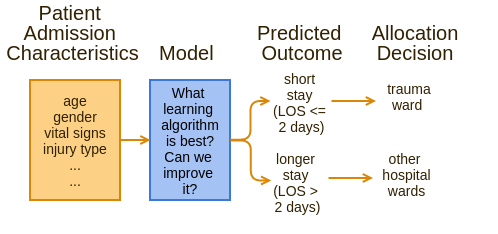
\includegraphics{problem-diag}
\end{center}

\noindent If we could accurately classify patients with hospital length of
stay (\los) of 2 days or less versus those who require longer stays, we could
make a more informed decision whether or not to place them in another ward
when they are admitted, rather than having to waste time and resources
transferring them to another ward later. This also frees up the high-demand
trauma beds for the critically injured who need them most.
\\

% =============================================================================
\section{Motivation}
\noindent Accurate prediction of the \los in various medical
domains (such as burns and acute pancreatitis) has been extensively studied,
as it is a key indicator of the level of
resource utilisation in hospitals and directly impacts the use of their limited
funding \cite{Walczak2003}.
\\

\noindent However, the current literature focuses extensively
on logistic regression and generalised linear models, with some applications
of techniques from machine learning such as artificial neural networks.
There has been no work done in systematically
applying a range of machine learning techniques to \los prediction, and
specifically not to the trauma medical domain.
\\

\noindent Additionally, there has been little work done in feature
transformation and selection when \los prediction models are created.
\\

% =============================================================================
\section{Contribution}
\noindent Building upon the work of trauma \los prediction in \cite{Dinh2013a},
we systematically investigate feature transformation and selection
techniques in the construction of a \los prediction model for trauma patients.
We also apply and evaluate a comprehensive range of
classification algorithms on data from the trauma domain as well as from a
general hospital setting.
\\

\noindent Additionally, we
propose a new nearest-neighbour (\nn) algorithm, ranked \nn, which takes
into account the
predictive relevance of features when computing the distance to the nearest
neighbours.
\\

% =============================================================================
\section{Datasets}
\noindent Our study was conducted on two datasets: one with 2546 records from
the Trauma Services Centre at the Royal Prince Alfred Hospital in Sydney,
consisting of
users admitted to the centre between 2007--11; the other from the Hospital das
Foras Armadas in Portugal with 17546 records collected from 2000--13.
\\

\noindent
The dataset from Sydney consists solely of patients admitted to Trauma
Services, whereas the dataset
from Portugal is a collection of hospital-wide inpatient admissions spanning
a range of diagnoses.
\\

% =============================================================================
\section{Approach}
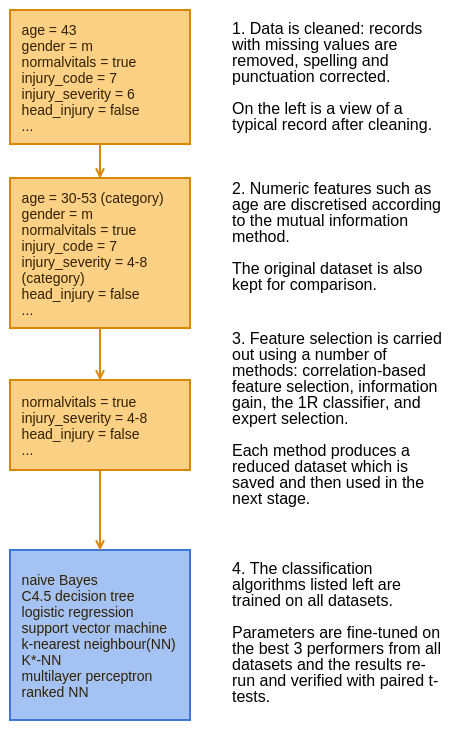
\includegraphics{approach}

\subsection{Ranked Nearest Neighbour}
\noindent \textit{Idea: the contribution of a feature to the distance between
two records should be proportional to its level of `relevance' or predictive
power with respect to the outcome variable, \los.} This is how it works:
\begin{center}
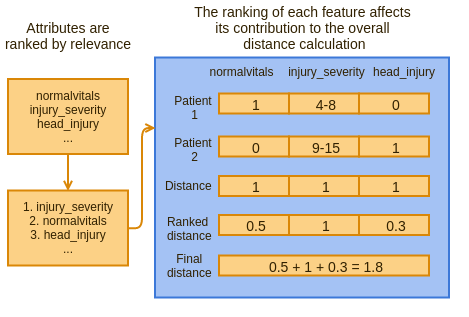
\includegraphics{ranked-nn}
\end{center}

% =============================================================================
\section{Evaluation Metrics}
\noindent \textit{Area under the receiver-operating characteristic curve (\auc)},
the extent to which the classification algorithm is able to distinguish between
patients that require a stay of less than 2 days or those who require longer.
Randomly picking between two outcomes has \auc 0.5, and the maximum is 1,
indicating perfect discriminating ability.
\\

\noindent Our \textit{baseline} is the logistic regression model derived in
\cite{Dinh2013a}, as we aim to improve upon the results they achieved for
trauma patients.
\\

\noindent All \auc figures are obtained from
\textit{10-fold stratified cross-validation}.
\\

% =============================================================================
\section{Results}
\noindent

% =============================================================================
\section{Conclusions and Future Work}
\noindent

% =============================================================================
\section{Acknowledgements}
\noindent
Many thanks to Dr Michael Dinh, co-director of Royal Prince Alfred
Hospital Trauma Services, for providing the trauma data and medical domain
guidance; and thanks also to Associate Professor Paulo Cortez, from the
Department of Information Systems at the University of
Minho in Portugal, for providing an extensive general \los dataset.
\\

% =============================================================================

\references
\bibliography{../thesis/references}

\end{multicols}
\end{document}
